\documentclass[border=10pt]{standalone}
\usepackage[left=25mm,right=25mm,top=25mm,bottom=25mm]{geometry}
\usepackage[utf8]{inputenc}
\usepackage[T1]{fontenc}
\usepackage{times}
\usepackage{geometry}
\usepackage{amsmath}
\usepackage{amssymb}
\usepackage{mathrsfs}
\usepackage{amsfonts}
\usepackage{amsthm}
\usepackage{lipsum}
\usepackage{amscd}
\usepackage{graphicx}
\usepackage{fancyhdr}
\usepackage{textcomp}
\usepackage{txfonts}
\usepackage[all]{xy}
\usepackage{paralist}
\usepackage[colorlinks=true]{hyperref}
\usepackage{array}
\usepackage{tikz}
\usepackage{slashed}
\usepackage{pdfpages}
\usepackage{cite}
\usepackage{url}
\usepackage{amsmath,amsfonts,amssymb}
\usetikzlibrary{shapes.geometric}
\usepackage{tikz}
\usetikzlibrary{automata,positioning}
\usepackage{listings}
\usepackage{multirow}
\usepackage{color}

\begin{document}



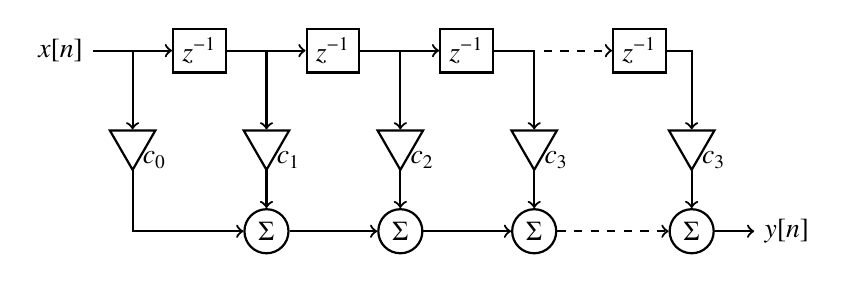
\begin{tikzpicture}

\draw[->,thick] node[anchor=east] {$x[n]$} (0,0) -- (1,0)
 node[anchor=west,draw,thick,minimum width=1,minimum height=1] (z1) {$z^{-1}$}  ;
\draw[->,thick] (z1.east) --++ (1,0)  node[anchor=west,draw,thick,minimum width=1,minimum height=1] (z2) {$z^{-1}$};
\draw[->,thick] (z2.east) --++ (1,0)  node[anchor=west,draw,thick,minimum width=1,minimum height=1] (z3) {$z^{-1}$};
\draw[thick] (z3.east) -- (5.6,0){};
\draw[->,thick, dashed] (z3.east) --++ (1.5,0) node[] (end) {};
\node[anchor=west,draw,thick,minimum width=1,minimum height=1] at (end) (z4) {$z^{-1}$};

\draw[->,thick] (0.5,0) -- (0.5,-1) node[isosceles triangle,
isosceles triangle apex angle=60,
draw, rotate=270, anchor=west,
minimum size=0.5cm] (t1) {} node[anchor=north west] at (t1) {$c_0$};
\node at (0.5,-1.5)  (test) {};
%  node[anchor=west,circle,draw,inner sep=2.5pt]{$\Sigma$};

\draw[->,thick] (2.2,0) -- (2.2,-1) node[isosceles triangle,
isosceles triangle apex angle=60,
draw, rotate=270, anchor=west,
minimum size=0.5cm] (t2) {} node[anchor=north west] at (t2) {$c_1$};
\draw[->, thick] (t2 |- test) --++ (0,-0.5) node[anchor=north,circle,draw,inner sep=2.5pt] (sigma) {$\Sigma$};

\draw[->, thick] (test.center) -- (test |- sigma) -- (sigma.west);

\draw[->,thick] (3.9,0) -- (3.9,-1) node[isosceles triangle,
isosceles triangle apex angle=60,
draw, rotate=270, anchor=west,
minimum size=0.5cm] (t3) {} node[anchor=north west] at (t3) {$c_2$};
\draw[->, thick] (t3 |- test) --++ (0,-0.5) node[anchor=north,circle,draw,inner sep=2.5pt] (sigma2) {$\Sigma$};

\draw[->, thick] (sigma.east) -- (sigma2.west);

\draw[->,thick] (5.6,0) -- (5.6,-1) node[isosceles triangle,
isosceles triangle apex angle=60,
draw, rotate=270, anchor=west,
minimum size=0.5cm] (t4) {} node[anchor=north west] at (t4) {$c_3$};
\draw[->, thick] (t4 |- test) --++ (0,-0.5) node[anchor=north,circle,draw,inner sep=2.5pt] (sigma3) {$\Sigma$};

\draw[->, thick] (sigma2.east) -- (sigma3.west);

\draw[thick] (z4.east) -- (7.613,0);

\draw[->,thick] (7.6,0) -- (7.6,-1) node[isosceles triangle,
isosceles triangle apex angle=60,
draw, rotate=270, anchor=west,
minimum size=0.5cm] (tn) {} node[anchor=north west] at (tn) {$c_3$};
\draw[->, thick] (tn |- test) --++ (0,-0.5) node[anchor=north,circle,draw,inner sep=2.5pt] (sigman) {$\Sigma$};

\draw[->, thick, dashed] (sigma3.east) -- (sigman.west);
\draw[->, thick] (sigman.east) --++ (0.5,0) node[anchor=west] {$y[n]$};

\end{tikzpicture}


\end{document}
